MongoDB ist ein in C++ geschriebenes, dokumentenorientiertes NoSQL-Datenbanksystem, das im Jahre 2009 von den Entwicklern Horowitz und Merriman als Open-Source Datenbank veröffentlicht wurde und die am weitest-verbreiteste NoSQL-Datenbank (Stand April 2021) \cite{DB1.7}. Die Intention der Gründer war es, eine Datenbank mit höherer Skalierbarkeit, Flexibilät und Performance zu entwerfen, die auf auf einer einfachen Handhabung beruht \cite{DB1.65}.
Gründe der Popularität der Datenbank ist neben den oben erwähnten Eigenschaften die flexible Gestaltungsmöglichkeit der Datenstrukturen sowie die Unterstützung durch zahlreiche Programmiersprachen und Betriebssysteme.
\noindent
Dem Konzept des CAP-Theorems folgend steht MongoDB für Konsistenz und Partitionstoleranz, dafür ordnet sich die Verfügbarkeit den anderen Eigenschaften unter.
\newline

\paragraph{Struktur}

\begin{figure}[tbt]
\centering
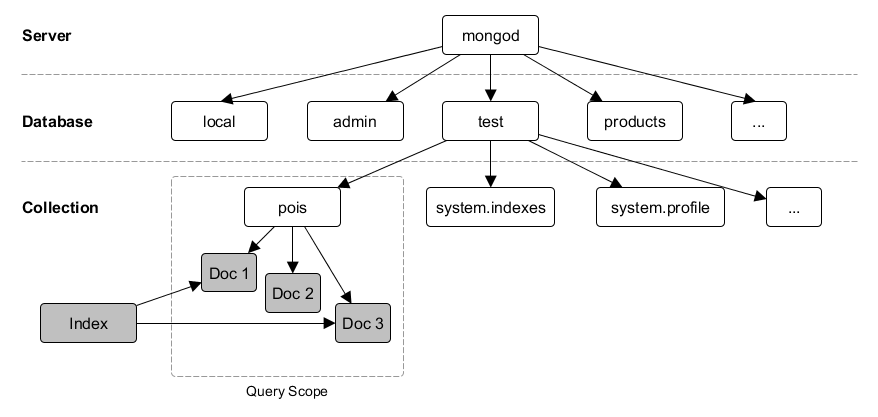
\includegraphics[width=14cm]{images/MongoDB_Architektur.png}
\caption[MongoDB Architektur]{MongoDB Architektur \protect \footnotemark}
\label{fig:MongoDBArchitektur}
\end{figure}
\footnotetext{\url{https://www.informatik-aktuell.de/betrieb/datenbanken/mongodb-fuer-software-entwickler.html}, letzter Zugriff: 9. Februar 2021}

\noindent
Die Abbildung \ref{fig:MongoDBArchitektur} stellt die grundsätzliche Struktur einer Mongo"-DB-"-Instanz dar.
Ein \textbf{Server} kann mehrere logische \textbf{Datenbanken} verwalten, die ihrerseits einen oder mehrere logische Namensräume enthalten, die sogenannten \textbf{Collections}. Eine Collection verwaltet die einzelnen Datensätze, die als \textbf{Dokumente} bekannt sind.  \\

\noindent
\textbf{Schema-Freiheit:}
Collections sind schemafrei. Dadurch gibt es für die zugehörigen Dokumente kein vorausgesetztes Schema. Aufgrund der Schema-Freiheut dürfen dennoch Architekturentscheidungen bei der Datenmodellierung nicht ignoriert werden. Stattdessen werden diese Entscheidungen des Schema-Managements auf die Anwendungsentwicklung verlagert. \\

\noindent
\textbf{BSON:}
Während MongoDB für Datenaustausch das JSON-Format nutzt, hält es seine Dokumente im Binary JSON-Format (BSON), einer binärcodiertem Erweiterung des JSON-Formats. Daten im BSON-Format enthalten zusätzlich Informationen zum Typ und zur Länge der Informationen, wodurch schnelleres Parsen von Daten möglich ist. Des Weiteren ist BSON um zusätzliche Datentypen wie 32- und 64-bit Integer oder das Datum erweitert \footnote{\url{https://www.mongodb.com/json-and-bson]}, letzter Zugriff: 12. Februar 2021}.

\begin{lstlisting}[caption=JSON - BSON Vergleich, label=lst:JSONBSON]
/* JSON */
{"hello": "world"}  // "key":"value"

/* BSON */
\x16\x00\x00\x00           // Gesamtgroesse des Dokuments
\x02                       // 0x02 = Typ String
hello\x00                  // Feldname
\x06\x00\x00\x00world\x00  // Feldwert
\x00                       // 0x00 = Typ EOO ('end of object')
\end{lstlisting}


\noindent
\textbf{ObjectID und Primärschlüssel:}
Für die eindeutige Identifikation eines Dokuments vergibt MongoDB automatisch erstellte '\_id'-Felder. Dabei wird bei der Generierung des BSON-Dokuments für den Wert das '\_id'-Feld ein Datentyp 'ObjectId\'  hinzugefügt. Dieses Identifikationsfeld ist gleichzusetzen mit den Primärschlüsseln aus relationalen Datenbanken \cite{DB1.85}. Ist eine automatische Generierung des eindeutigen Identifikationsfeldes nicht erwünscht, kann der Anwendungsentwickler dieses Feld auch selbst erzeugen, indem er die Eigenschaft explizit dem zu erstellenden Objekt hinzufügt und mit einem Wert verseht.
\newline

\paragraph{Datenbankabfrage}
Im Vergleich zu relationalen Datenbanken benutzt MongoDB keine Abfragesprache wie SQL. Stattdessen ermöglicht dieses Datenbanksystem drei Arten von Abfragen, wobei eine Abfrage sich immer auf genau eine Collection bezieht. Ein Bezug einer Abfrage zu mehreren Collections, wie es relationale Datenbanken mit „Join“-Operationen erlauben, ist hier nicht gegeben und muss in der Anwendung realisiert werden \cite{1.9}. Abfragen in MongoDB werden grundsätzlich in Form von Dokumenten formuliert. Dieses Verfahren ermöglicht schnelles Abhandeln komplexer Abfragen von tief geschachtelten Dokumentenstrukturen. Nachfolgend werden die drei Abfragemöglichkeiten erläutert.

\noindent
\textbf{Query-By-Example:}
Das folgende Beispiel zeigt einen Aufruf aller Einträge, die als Ort Karlsruhe eingespeichert haben. 
\newline
\begin{lstlisting}[caption=MongoDB Read, label=lst:MongoDBRead]
db.pois.find( {"adresse.ort": "Karlsruhe" } )
\end{lstlisting}

\noindent
Dabei kommt das Prinzip Query-by-Example \footnote{Query By Example: \url{https://de.wikipedia.org/wiki/Query_by_Example}, letzter Zugriff: 12. Februar 2021} zum Einsatz, bei dem die als JSON-Dokument beschriebenen Suchkriterien als Filter auf die durchsuchte Collection wirkt. Zusätzlich stehen für diese Art von Abfragemöglichkeit sämtliche logische Verknüpfungen und Vergleichsoperatoren zur Verfügung\footnote{Query-Operatoren\url{https://docs.mongodb.com/manual/reference/operator/query/}, letzter Zugriff: 12. Februar 2021}.
Das Ergebnis der obigen Find-"-Operationen liefert dabei einen Cursor zurück, über den die aufrufende Anwendung durch die einzelnen zurückgelieferten Dokumente iterieren kann. Außerdem kann der Cursor modifiziert werden, um beispielsweise Beschränkungen der Trefferanzahl oder Sortierung vorzunehmen. \\

\begin{lstlisting}[caption=MongoDB Read Modifikation, label=lst:MongoDBReadModifikation]
db.pois.find().limit(5).sort({"adresse.ort": -1})
\end{lstlisting}

\noindent
\textbf{MapReduce:}
MapReduce ist ein allgmeines Programmiermodell zur verteilten und parallelen Verarbeitung von großen Datenmengen in aggregierte Ergebnisse. Dabei unterteilt sich der Algorithmus im Wesentlichen in zwei Operationen \footnote{MapReduce Dokumentation \url{https://docs.mongodb.com/manual/core/map-reduce/}, letzter Zugriff: 10. Februar 2021}:
\newline
-	Map: Emittieren der beliebig vielen Key-Value-Paare für jedes Dokument
\newline
-	Reduce: Zusammenfassen aller Daten, die einem Kriterium entsprechen.\\

\noindent
\textbf{Aggregation-Framework:}
Das Aggregation-Framework bietet als Alternative zum MapReduce-Verfahren den Vorteil der besseren Performance\footnote{\url{https://docs.mongodb.com/manual/meta/aggregation-quick-reference/}, letzter Zugriff: 14. Februar 2021}. Dabei wird eine Pipeline genutzt, die das resultierende Dokument einer Operation an die Eingabe der nächsten Operation weiterleitet. Die entsprechende Funktion ist die Aggregate()-Operation, deren Parameter als Array von Dokumenten die Pipeline-Operatoren abbilden . Tabelle \ref{tab:AggregationFrameworkPipelineOperatoren} zeigt die zur Verfügung stehenden Pipeline-Operatoren.\\

\begin{lstlisting}[caption=MongoDB Aggregate, label=lst:MongoDBAggregate]
db.pois.aggregate([
    {$group: {_id: "$adresse.ort", n: {$sum:1}}},
    {$sort: {n: -1}}
])
\end{lstlisting}

\begin{table}[h]
\caption[Aggregation Framework: Pipeline-Operatoren]{Aggregation Framework: Pipeline-Operatoren [MongoDB1.9]}
\label{tab:AggregationFrameworkPipelineOperatoren}
\begin{center}
    \begin{tabular}{ l  p{12cm}}
    \toprule
    \textbf{Operator}  & \textbf{Beschreibung} \\
    \midrule
\rule{0pt}{17pt}
    \$match &Sucht Dokumente analog zu find(). Sollte idealerweise mindesten 1x zu Beginn der Pipeline ausgeführt werden, um die Ergebnismenge einzuschränken.\\
    
\rule{0pt}{17pt}
    \$project & Schränkt auf eine Teilmenge von Feldern ein und verändert die Feldwerte.  \\
    
\rule{0pt}{17pt}
	\$sort & Sortiert die Dokumente. Analog zu sort() bei find(). .\newline
	Benötigt Private Key und Zertifikat.  \\
	
\rule{0pt}{17pt}
    \$skip & Überspringt n Dokumente. Analog zu skip() bei find().  \\ 
    
\rule{0pt}{17pt}
    \$limit & Begrenzt auf n Dokumente. Analog zu limit() bei find().  \\

\rule{0pt}{17pt}
   \$group   &	Gruppiert nach einem oder mehreren Feldern. \\ 

\rule{0pt}{17pt}
	\$unwind  &	Wird auf ein Array angewendet. Jeder Array-Eintrag generiert dann ein neues Dokument für die nächste Pipeline-Stufe.\\

\rule{0pt}{17pt}
	\$redact  &	Filtert Felder des Dokuments in Abhängigkeit vom Inhalte anderer Felder.\\

\rule{0pt}{17pt}
	\$out  &	Leitet das Ergebnis der Aggregation in eine Collection um. Kann nur als letzter Operator verwendet werden.  \\
    \bottomrule
    \end{tabular}
\end{center}
\end{table}
\footnotetext{\url{https://www.informatik-aktuell.de/betrieb/datenbanken/mongodb-fuer-software-entwickler.html}, letzter Zugriff: 9. Februar2021}



\paragraph{CRUD}
MongoDB unterstützt eine Vielzahl an Operationen zum Erzeugen, Lesen, Updaten und Löschen von Daten.
Tabelle \ref{CRUDOperatoren} stellt die Kommandos zur Realisierung der CRUD-Operationen in MongoDB dar.
\newline

\begin{table}[tbt]
\caption{CRUD-Operatoren}
\label{CRUDOperatoren}
\begin{center}
    \begin{tabular}{ l  p{8cm}  l }
    \toprule
    \textbf{Operation} & \textbf{Beschreibung} & \textbf{MongoDB Methode} \\
    \midrule

    Create & Datensätze erstellen & .Insert() \\

	Read & Datensätze lesen & .Find() \\

    Update & Daten aktualisieren & .Update() \\ 

    Delete & Datensätze entfernen & .Remove()  \\ 
    \bottomrule
    \end{tabular}
\end{center}
\end{table}

\noindent
\hangindent1cm
\textbf{Create:}
„InsertOne()“ erzeugt ein einzelnes Dokument in der jeweiligen Collection der Datenbank. Dabei wird ein Dokument im JSON-Format als Parameter mitgegeben. ObjectID wird, wenn nicht als Eigenschaft im Dokument angegeben, automatisch von MongoDB erzeugt. Ebenfalls wird die angesprochene Collection automatisch erzeugt, falls sie nicht bereits existiert. Die Funktion „InsertMany()“  erlaubt das Hinzufügen mehrerer Datensätze über ein Array von JSON-Dokumenten als Parameter. Die Methode „Insert“ ist flexibler und bietet beide Parametrisierungsmöglichkeiten\footnote{\url{https://docs.mongodb.com/manual/reference/method/db.collection.insert/\#mongodb-method-db.collection.insert}, letzter Zugriff: 14. Februar 2021}.
\newline
\begin{lstlisting}[caption=MongoDB Create, label=lst:MongoDBCreate]
db.personen.insertOne({"vorname" : "Robin"});
\end{lstlisting}

\noindent
\hangindent1cm
\textbf{Read:}
Um Datensätze aus der Datenbank zu lesen, wird die find()-Methode zur Verfügung gestellt. Sie gibt alle Dokumente einer Kollektion zurück. Wie im Kapitel Query-By-Example beschrieben, kann die Funktion mit Filtern versehen werden. Die Funktion findOne() bietet die gleiche Funktionsweise, die Dokumentenausgabe ist aber auf ein einzelnes Dokument begrenzt. 
Ein Beispiel ist dargestellt in Listing \ref{lst:MongoDBRead}.
\newline\newline

\noindent
\hangindent1cm
\textbf{Update:}
Die Update()-Methode ermöglicht es, Änderungen an Datensätzen vorzunehmen.  Die Methode erhält zwei Parameter, einen zur Angabe der gesuchten Dokumente und den anderen mit  der vorzunehmenden Änderung. Simultan zu den Insert-Methoden gibt es die UpdateOne()-Methode für Änderungen an einem Dokument und UpdateMany()-Methode für mehrere Dokumente.
\newline

\begin{lstlisting}[caption=MongoDB Update, label=lst:MongoDBUpdate]
db.personen.updateOne({"vorname" : "Robin"} , currentDate("last_login") );

\end{lstlisting}

\noindent
\hangindent1cm
\textbf{Delete:}
Für das Löschen von Datensätzen aus einer Collection gibt es die DeleteOne()- und DeleteMany()-Methode. Über mitgegegeben Parameter können Filter eingestellt werden. Eine ganze Collection kann mit der drop()-Methode entfernt werden.
\newline

\begin{lstlisting}[caption=MongoDB Remove, label=lst:MongoDBRemove]
db.personen.deleteOne( {"vorname" : "Robin"} );

\end{lstlisting}

\noindent
\paragraph{Atomare Operationen}
Als atomare Operationen wird ein Verbund von Einzeloperationen bezeichnet, der als logische Einheit betrachtet wird und nur als Ganzes erfolgreich abläuft oder fehlschlägt. In Bezug auf Datenbanken spricht man von Transaktionen, die entweder als Ganzes erfolgreich ablaufen (Commit) oder nach einer fehlerhaften Einzeloperation rückgangig gemacht werden (Rollback). Ohne atomare Operationen können Probleme aufkommen, die zu einer Inkonsistenz der Datenzustände führt. Beispielsweise würde ein Abbruch inmitten mehrerer zusammenhängender Operationsabläufe dazu führen,  dass nur ein Teil der Operationen ausgeführt wurde, während die restlichen Operationen und somit die verbleibenden Datenänderungen verworfen werden.
\newline
Bis vor dem Jahre 2018 unterstützte MongoDB keine Transaktionen. Mit der Veröffentlichung der Version 4.0 wurde der Funktionsumfang von MongoDB stark erweitert. Eines der neuen Erweiterungen war die Möglichkeit, Transaktionen durchführen zu können. Dafür werden sogenannte „Sessions“ genutzt. Sämtlichen CRUD-Operationen, die einer Transaktion zugehören sollen, werden eine Session als zusätzlicher Parameter hinzugefügt.  Bei Abschluss der Transaktion kann sie mit der Methode „session.commitTransaction()“ bestätigt werden. Andernfalls, sollte ein Fehler aufgetreten sein, kann die Methode „session.abortTransaction()“ die Operationen rückgängig machen. Eine wichtige Vorraussetzung, um Transaktionen in MongoDB nutzen zu können, ist ein Replica Set aufzusetzen. Darauf wird im weiteren Kapitel eingegangen. 
\newline


\paragraph{Architektur}
Bei der Inbetriebnahme einer MongoDB Datenbank spielen zwei Prozesse eine wichtige  Rolle. \newline Der  „mongod“-Prozess ist der primäre Hintergrundprozess für das Datenbanksystem. Er behandelt Datenabfragen, Datenzugriffe und führt benötigte Hintergrundoperationen durch\footnote{Mongod \url{https://docs.mongodb.com/manual/reference/program/mongod/}, letzter Zugriff: 15. Februar 2021}. Beim Starten des mongod-Prozesses können über Flags Konfigurationen vorgenommen werden, beispielsweise ändert „--port 5000“ den Port. Nach erfolgreichem Start des Prozesses kann über den Standard Port der MongoDB (27017) bzw. über den konfigurierten Port eine Verbindung hergestellt werden.\newline
Der Prozess, der als Controller für sich auf mehreren Datenbanken befindenden verteilte Daten dient, nennt sich „mongos“\footnote{Mongos \url{https://docs.mongodb.com/manual/reference/program/mongos/}, letzter Zugriff: 15. Februar 2021}. Dieser Prozess findet seinen Einsatz hauptsächlich in Kombination mit Sharding, auf die im weiteren Unterkapitel eingegangen wird. \newline

\noindent
\hangindent1cm
\textbf{Engine:}
Als Storage Engine, oder auch Datenbank-Engine, wird die zugrundeliegende Softwarekomponente eines Datenbanksystems zum Verwalten der Daten bezeichnet. Die gebräuch"-lich"-sten Engines in MongoDB sind die MMAPv1-Engine und die WiredTiger-Engine.\newline
Bis vor Version 3.2 war MMAPv1-Engine die Standard-Storage Engine von MongoDB. Eine Kompression der Daten wurde nicht unterstützt und Transaktionen waren nur auf einem Dokument ausführbar. Ab MongoDB 3.2 wird standardmäßig die Wired Tiger-Engine eingesetzt. Neben der Kompression der Daten und der miteingehenden Verringerung des benötigten Speicherplatzes bietet diese Engine auch eine Verschlüsselung der Daten an. Abhängig des benutzten Kompressionsalgorithmus kann der benötigte Verbrauch um 70\% für Daten und um 50\% für Indizes reduziert werden \cite{DB3.5}. Die WiredTiger-Engine skaliert im Vergleich zur MMAPv1 mit der Anzahl der CPU-Kerne und ermöglicht Transaktionen über mehrere Dokumente hinweg. Die genutzte Engine kann in den Konfigurationen eingestellt werden.
\newline

\noindent
\hangindent1cm
\textbf{Replica Sets:}
Im standardmäßigen Standalone-Modus besteht bei Ausfall des Servers die potenzielle Gefahr des Datenverlusts. Das Problem lässt sich durch Replikation beheben. Hierbei spricht man von der bloßen Herstellung von Mehrexemplaren(Kopien) derselben Daten, die meistens regelmäßig abgeglichen werden \cite{DB3.6}. MongoDB realisiert die Replikation der Daten über Replica Sets\cite{DB3.7}. Dabei handelt es sich um eine Gruppe von mongod-Prozessen, die dieselben Daten enthalten. Nach dem CAP-Theorem ist MongoDB nicht auf Verfügbarkeit ausgelegt. Dennoch umgeht die Datenbank diesen Nachteil über die Anwendung von Replica Sets. Das Replica Set besteht aus einem primären Knoten und daraus replizierenden Sekundären Knoten.
Nur der primäre Knoten führt datensatzändernde Operationen aus. Veränderungen werden in sogenannten 'Oplogs' (Operations logs) gespeichert, die zum Austausch der Daten innerhalb des Replica Sets genutzt wird \cite{DB3.8}. Bei den Oplog-Dateien handelt es sich um Collections mit festgelegten Speichergrößen, den sogenannten „capped collections“. Während die Oplog-Dateien ähnlich wie ein Logbuch mit allen Veränderungen in den Datensätzen der Datenbank beschrieben werden, werden bei erreichter Maximalgröße der Collection die ältesten Daten von den neuen Daten überschrieben. Dabei enthält jeder Knoten des Replica Sets seine eigene Kopie des Oplogs und gleicht ihn mit dem des primären Knotens ab. Das Konzept der Replica Sets wird in Abbildung \ref{fig:ReplicaSet} dargestellt.

\begin{figure}[tbt]
\centering
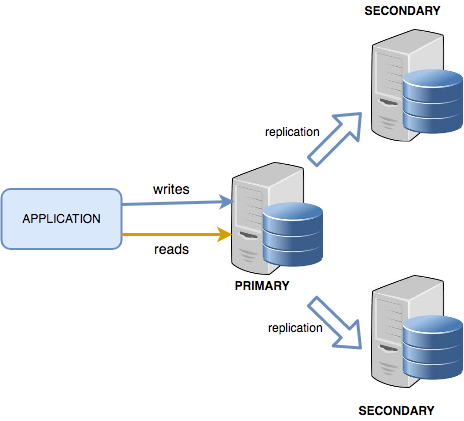
\includegraphics[width=7cm]{images/replicaset1.png}
\caption{MongoDB Replica Set}
\label{fig:ReplicaSet}
\end{figure}
\footnotetext{Bild aus \cite{DB3.8}}


\noindent
\hangindent1cm
\textbf{Sharding:}
Hierbei ist die Rede von der Methodik zur Aufteilung der Daten auf mehrere Datenbanken \cite{DB4.1}.
Der Datenbestand wird nach logischen Kriterien in  Teilstücke, die sogenannten „Shards“, zerlegt und über mehrere Replica Sets verteilt.
In Hinblick auf das hinzufügen weiterer Server gewährt das Sharding eine horizontale Skalierbarkeit.
Des Weiteren werden durch die Tatsache, dass jeder Shard für seinen Bestandteil zuständig ist,  Suchanfragen schneller durchgeführt. 
Sharding ist besonders bei großen Datenmengen in Bezug auf Performance von Vorteil.
Der mongos-Prozess leitet Anfragen an die jeweiligen Shards weiter und dient als Schnittstelle zwischen den Clientanwendungen.

\paragraph{Verwaltungswerkzeuge}
\noindent
\hangindent1cm
\textbf{Mongo Shell:}
Der „mongo“-Prozess ist eine interaktive JavaScript Schnittstelle auf der Kommandozeile. Er bietet umfassende Funktionalitäten für die Systemadministration des Datenbankensystems als auch Zugriff auf die Datensätze\footnote{Mongo \url{https://docs.mongodb.com/manual/reference/program/mongo/}, letzter Zugriff: 15. Februar 2021}. Dazu erhält man eine Eingabeaufforderung, auf dem Befehle in der Sprache JavaScript ausgeführt werden können.
\noindent
\hangindent1cm
\textbf{Treiber:}
MongoDB bietet für viele Programmiersprachen bzw. Frameworks Softwarebibliotheken zum Zugriff auf die Datenbank an.\footnote{MongoDB Treiber \url{https://docs.mongodb.com/drivers/}, letzter Zugriff: 01. Mai 2021}  Eine offiziell unterstützte ist Mongoose für das Node.js-Framework\footnote{Mongoose - Offizielle Webpage \url{https://mongoosejs.com/docs/}, letzter Zugriff: 01. Mai 2021}
\newpage
\noindent
\hangindent1cm
\textbf{Grafische Oberflächen:}
Es gibt einige Anwendungen zur visuellen Darstellung und Bearbeitung der Datenbanken in MongoDB, die eine grafische Benutzeroberfläche bieten. Zum Beispiel MongoDB Compass, Studio3T oder Fang of Mongo. In Abbildung \ref{MongoDBCompass} wird die Benutzeroberfläche von MongoDBCompass dargestellt


\begin{figure}[tbt]
\centering
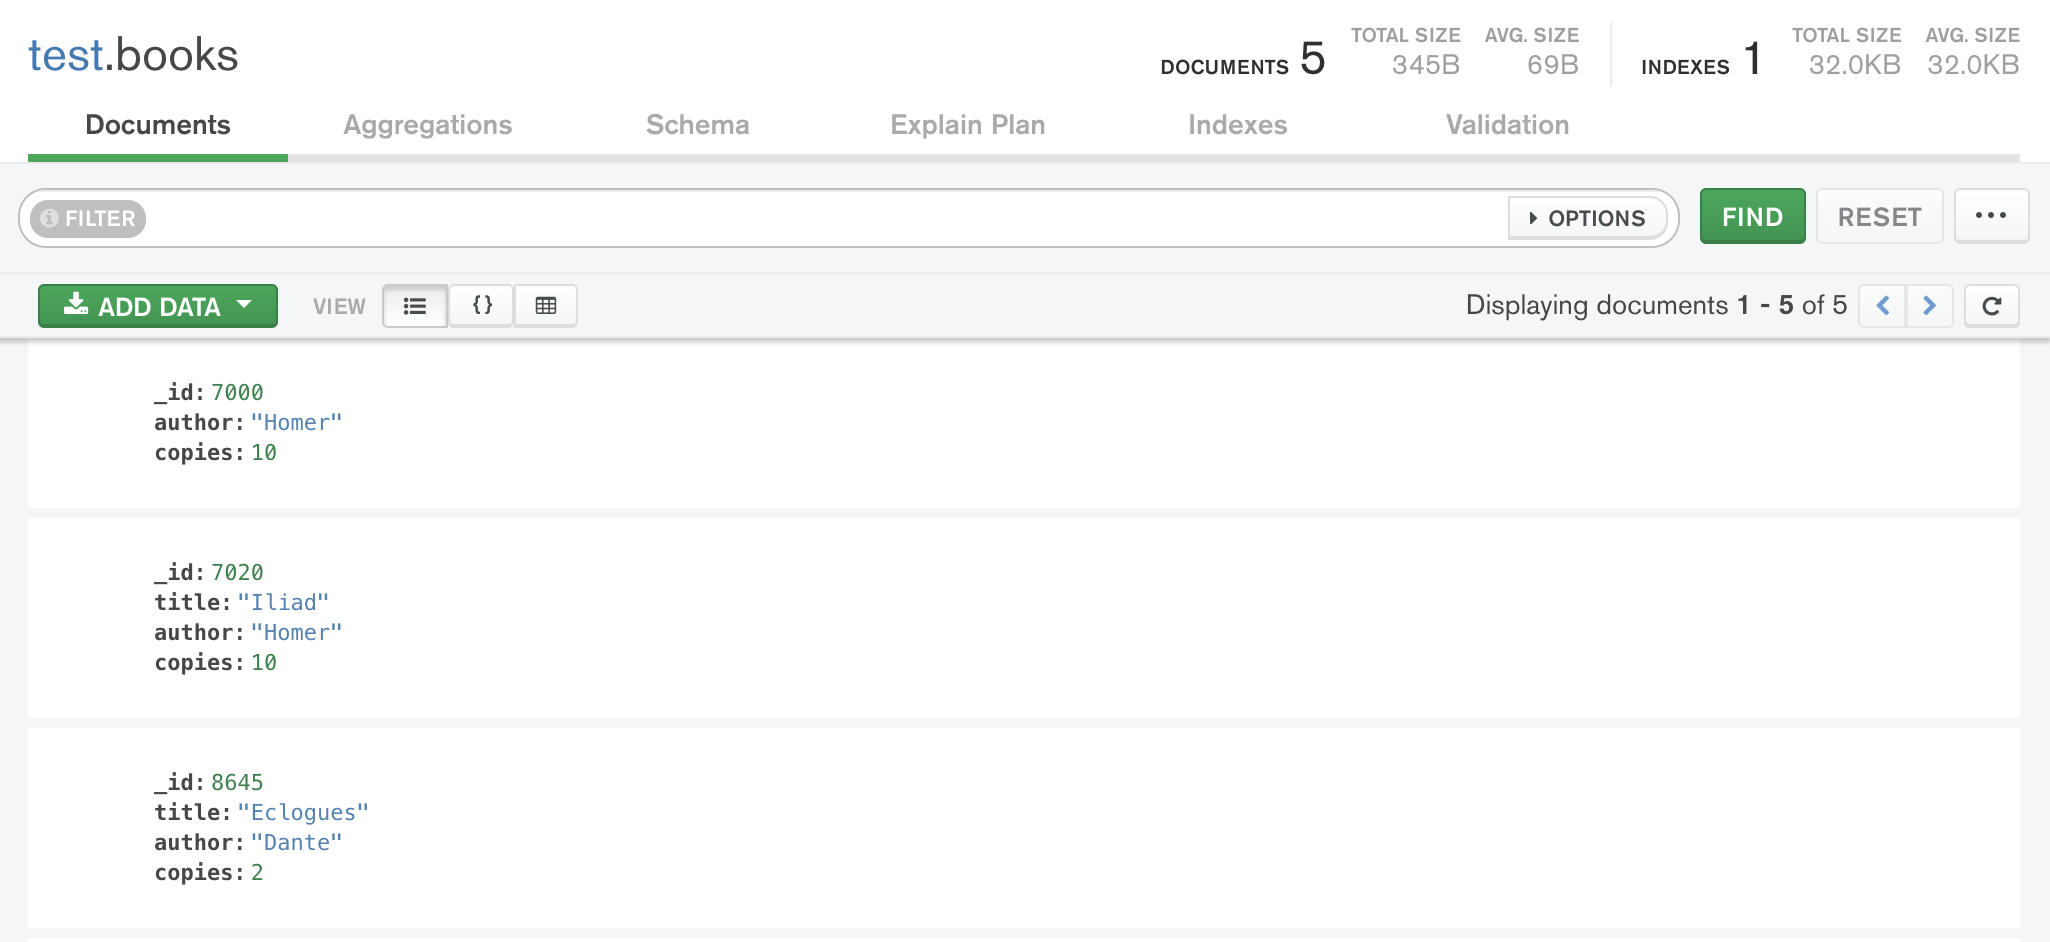
\includegraphics[width=15cm]{images/mongodb_compass.png}
\caption{MongoDBCompass Benutzeroberfläche}
\label{MongoDBCompass}
\end{figure}